The \emph{cosmic microwave background radiation}, as we explained in section \ref{sec:LambdaCDM}, is one of the most valuable source of information that we got from the early universe. Its usefulness is encoded in its \textbf{anisotropies}: the small variations, in its temperature for example, from the perfectly homogeneous radiation that we would have in absence of perturbations. Anisotropies thus are a direct link to the perturbations that were generated in the early universe and allow us to obtain data from the earliest stages of the universe, such as inflation. To begin we will consider scalar perturbations, then we will also develop the same machinery for the tenosr one.
\section{Angular power spectrum}\label{sec:AngularPowerSpectrum}
When we observe the \emph{CMB} in the sky, we measure the temperature of photons coming from a specific direction $\mathbf{\hat{n}}$ to us. As we know, this temperature is not perfectly the same from all directions, we call these tiny differences \emph{anisotropies}:
$$T(\mathbf{\hat{n}}) = \bar{T} \left[1 + \Theta(\mathbf{\hat{n}})\right] \qquad \text{with } \Theta(\mathbf{\hat{n}}) \stackrel{\text{def}}{=} \frac{\Delta T(\mathbf{\hat{n}})}{\bar{T}}$$
and where $\bar{T}$ is the average temperature in the sky and $\Delta T(\mathbf{\hat{n}})$ is the temperature fluctuation in the direction $\mathbf{\hat{n}}$.
To compare the temperature at two district points in the sky we define the \emph{two point correlation function}:
\begin{equation} \label{eq:ani2pcf}
    C(\mathbf{\hat{n}},\mathbf{\hat{n}}') \defeq \langle \Theta(\mathbf{\hat{n}})\Theta(\mathbf{\hat{n}}') \rangle,
\end{equation}
here the angle brackets denote an average over an ensemble of universes (It will be discussed later in this section how we can approximate this averaging process).


The most appropriate way to describe the temperature fluctuations, given that these are observed from the sky, is to expand $\Theta$ in spherical harmonics
\begin{equation}\label{eq:harmexpansion}
    \Theta(\mathbf{\hat{n}}) = \sum_{\ell=0}^{\infty} \sum_{m=-\ell}^{\ell} a_{\ell m} Y_{\ell m}(\mathbf{\hat{n}}),
\end{equation}
where the coefficients $a_{\ell m}$, also called \textbf{multipole moments}, are given by
\begin{equation*}
    a_{\ell m} = \int d\Omega\ \Theta(\mathbf{\hat{n}}) Y^*_{\ell m}(\mathbf{\hat{n}}).
\end{equation*}
Also, for the multipole moments we can define a two point correlation function
\begin{equation}\label{eq:angularpowerspectrum}
    \langle a_{\ell m} a^*_{\ell' m'} \rangle = \delta_{\ell \ell'} \delta_{m m'}\ C_{\ell},
\end{equation}
where $C_{\ell}$ is the \textbf{angular power spectrum} and again the angle brackets represent an ensemble average. Sometimes it is also used $\mathcal{D}_\ell \defeq \frac{\ell(\ell+1)}{2\pi}\bar{T}^2C_{\ell}$.

Note that combining \eqref{eq:harmexpansion} and \eqref{eq:ani2pcf} we obtain
\begin{align*}
    C(\mathbf{\hat{n}},\mathbf{\hat{n}}') &= \langle \Theta(\mathbf{\hat{n}})\Theta(\mathbf{\hat{n}}') \rangle \\ &= \sum_{\ell=0}^{\infty} \sum_{m=-\ell}^{\ell}  \sum_{\ell'=0}^{\infty} \sum_{m'=-\ell'}^{\ell'} \langle a_{\ell m} a_{\ell' m'} \rangle Y_{\ell m}(\mathbf{\hat{n}})Y_{\ell' m'}(\mathbf{\hat{n}}')\\
    &= \sum_{\ell=0}^{\infty}C_{\ell} \sum_{m=-\ell}^{\ell}  Y_{\ell m}(\mathbf{\hat{n}})Y^*_{\ell m}(\mathbf{\hat{n}}')\\
    &\ \Bigg\downarrow\quad \text{using } \sum_{m=-\ell}^{\ell}Y_{\ell m}(\mathbf{\hat{n}})Y^*_{\ell m}(\mathbf{\hat{n}}')=\frac{2\ell+1}{4\pi}P_{\ell}(\cos\theta)\\
    &=\sum_{\ell=0}^{\infty} C_{\ell}\frac{2\ell+1}{4\pi}P_{\ell}(\cos\theta),
    \end{align*}
where $P_{\ell}$ are the Legendre polynomials and $\theta$ is the angle between $\mathbf{\hat{n}}$ and $\mathbf{\hat{n}}'$.
Invoking the orthogonality of the Legendre polynomials we can write
\begin{equation}\label{eq:cl}
    C_{\ell} = 2\pi\int_{-1}^{1}d(\cos\theta)\ P_{\ell}(\cos\theta)C(\mathbf{\hat{n}},\mathbf{\hat{n}}'),
\end{equation}
this shows that the angular power spectrum encodes the same information as the two point correlation function \eqref{eq:ani2pcf}, hence it measures the correlation between the temperature fluctuations at two points in the sky separated by an angle $\theta$.

We now want to understand how can we estimate the average over the ensemble of universes in the previous definitions. Note that, fixed $\ell$, we still get $2\ell+1$ different values of $a_{\ell  m}$, this allows us to estimate the angular power spectrum as
\begin{equation}\label{eq:cl_estimate}
    \hat{C}_{\ell} = \frac{1}{2\ell+1}\sum_{m=-\ell}^{\ell} |a_{\ell m}|^2.
\end{equation}
One can show that this estimator is unbiased\footnote{An estimator is said to be unbiased if its expected value is equal to the true value of the parameter being estimated.}, however its variance is non-zero:
\begin{equation}\label{eq:cl_variance}
    \Delta\hat{C}_{\ell} \defeq\sqrt{\langle(C_\ell -\hat C_\ell)^2\rangle} = \sqrt{\frac{2}{2\ell+1}}C_{\ell},
\end{equation} 
this error that systematically appears in this estimate is usually called \textbf{cosmic variance}. Cosmic variance will result in a larger error for smaller values of $\ell$, which corresponds to larger angular scales. This can be understood as a consequence of the fewer number of modes $a_{\ell m}$ available at lower $\ell$.

\subsection{Multipole expansion}\label{sec:MultipoleExpansion}
In the previous section we considered the temperature fluctuations observed by us in the sky, therefore it was natural to assume that these were functions of the direction of observation $\versor n$. In general however, we should consider that these anisotropies varies also with the position of the observer in spacetime. This broader view is needed since to predict the observations we will need to describe the evolution of the anisotropies throughout the whole universe. Therefore, we will now consider
\begin{equation}
    \Theta({t,\mathbf x,\versor p})\quad\text{with}
    \begin{cases}
        t\quad\text{cosmic time,}\\
        \mathbf x\quad\text{position of the anisotropy in space,}\\
        \versor p\quad\text{direction of motion of the photons}.
    \end{cases}
\end{equation}
To come back to the observed anisotropies we just fix $t$ at the present day, $\mathbf x$ on the earth and we consider the direction of motion of the photons as the direction of observation (since it is the direction from which they come from).\\

In section \ref{sec:ThetaTimeEvolution} we will see that the evolution of the anisotropies is described by a linear differential equation (since we are working with first order perturbations). It is therefore useful to introduce here some expansions that will simplify these equations.\\
First of all, we can simplify the spacial dependence moving to Fourier space
\begin{equation}\label{eq:fourier_expansion}
    \Theta(t,\mathbf x,\versor p) = \int \frac{d^3k}{(2\pi)^3}e^{i\mathbf{k}\cdot\mathbf{x}}\tilde\Theta(\mathbf{k},t,\versor p),
\end{equation} 
where $\tilde\Theta$ is the Fourier transform of $\Theta$.
In this way, we obtained a decomposition on plane waves that leaves $\tilde\Theta$ depending on two vectors, $\mathbf k$ and $\versor p$. However, when dealing with the anisotropies generated only by \emph{scalar perturbations}\footnote{For tensor perturbations this expansion is not appropriate anymore, this is discussed in section \ref{sec:Anisotropies_From_Tensor}}, as we will see in section \ref{sec:ThetaTimeEvolution} the quantities that really matter are encoded in one of these two vectors and in the angle between them. This allows us to define $$\mu=\frac{\mathbf{k}\cdot \versor p}{k}\qquad\Rightarrow\qquad \tilde\Theta(t,\mathbf k,\mu)\quad \text{with } \mu\in[-1,1].$$
This suggests us to that another useful expansion is the \textbf{Legendre polynomial expansion}:
\begin{align}\label{eq:legendre_expansion}
    &\tilde\Theta(t,\mathbf k,\mu) = \sum_{\ell=0}^{\infty}\frac{2\ell+1}{i^\ell} \tilde\Theta_{\ell}(t,\mathbf{k})P_{\ell}(\mu),\\
    &\tilde\Theta_{\ell}(t,\mathbf{k}) =\frac{i^\ell}{2} \int_{-1}^{1}d\mu\ P_{\ell}(\mu)\tilde\Theta(t,\mathbf k,\mu)\nonumber,
\end{align} 
where $P_{\ell}$ are the Legendre polynomials and $\tilde\Theta_\ell$ are the \textbf{multipoles}.\\
The Legendre polynomials can be computed recursively using the Bonnet's formula
\begin{equation}\label{eq:bonnet}
    (\ell+1)P_{\ell+1}(\mu) = (2\ell+1)\mu P_{\ell}(\mu)-\ell P_{\ell-1}(\mu),
\end{equation}
and knowing that $P_0=1$, $P_1=\mu$ and $P_2=\frac{3\mu^2-1}{2}$.
\subsection{From perturbations to anisotropies}\label{sec:PertToAnis}
It is now time to discuss how in general we connect the perturbations of the FRW universe to the angular power spectrum of the anisotropies that we observe in the \emph{CMB}. Even though we will not study, in this work, the anisotropies themselves, this connection will be used, in a similar manner, when dealing with spectral distortions in the next chapter. 

We are interested in evaluating $\langle\tilde\Theta(\mathbf{k},\versor n)\tilde\Theta(\mathbf{k}',\versor n')\rangle$. This quantity is determined by two phenomena:
\begin{enumerate}
    \item the initial amplitude of the perturbations generated during inflation, which from our point of view are random variables generated by vacuum fluctuations;
    \item the evolution the anisotropies that we observe today and how they are sourced by the primordial perturbations: this process is clearly deterministic. 
\end{enumerate}
This consideration allows us to proceed in the following way: considering a generic primordial perturbation $\delta(\mathbf{k})$, we can decompose $ \tilde\Theta(\mathbf{k},\versor n)=\delta (\tilde\Theta/\delta) $, now the ratio $\tilde\Theta/\delta$ is completely independent of the initial amplitude of the perturbation (by initial conditions also $\Theta$ is proportional to this amplitude) and won't contribute to the ensemble average.\\
In this way we get
\begin{align*}
    \langle\tilde\Theta(\mathbf{k},\versor n)\tilde\Theta^*(\mathbf{k}',\versor n')\rangle &= \langle\delta(\mathbf{k})\delta(\mathbf{k}')\rangle\frac{\tilde\Theta(\mathbf{k},\versor n)}{\delta(\mathbf{k})}\frac{\tilde\Theta^*(\mathbf{k}',\versor n')}{\delta^*(\mathbf{k}')}\\
    &= (2\pi)^3\delta^{(3)}(\mathbf{k}-\mathbf{k}')\mathcal P_{\delta}(k)\frac{\tilde\Theta(\mathbf{k},\versor n)}{\delta(\mathbf{k})}\frac{\tilde\Theta^*(\mathbf{k}',\versor n')}{\delta^*(\mathbf{k}')},
\end{align*}
where we used the definition of the primordial perturbation power spectrum. In this expression the last two factors now depend only on the magnitude of $\mathbf k$ and $\mathbf k'$.\\Now, by inserting this result in the expression for the $C_\ell$ \eqref{eq:cl} we find 
\begin{align}
    C_{\ell}&=2\pi\int_{-1}^{1}d\mu P_{\ell}(\mu)\int\frac{d^3k}{(2\pi)^3}\int\frac{d^3k}{(2\pi)^3}e^{i(\mathbf k-\mathbf k')\cdot \mathbf x}\langle\tilde\Theta(\mathbf k,\versor n)\tilde\Theta^*(\mathbf k',\versor n')\rangle\nonumber\\
    &=2\pi\int\frac{d^3k}{(2\pi)^3}\mathcal P_{\delta}(k)\int_{-1}^{1}d\mu P_{\ell}(\mu)\frac{\tilde\Theta(\mathbf{k},\versor n)}{\delta(\mathbf{k})}\frac{\tilde\Theta^*(\mathbf{k},\versor n')}{\delta^*(\mathbf{k})}\nonumber\\
    &=2\pi\int\frac{dk\ k^2}{(2\pi)^3}\mathcal P_{\delta}(k)\int_{-1}^{1}d\mu P_{\ell}(\mu)\sum_{\ell',\ell''}\frac{\tilde\Theta_{\ell'}}{\delta}\frac{\tilde\Theta_{\ell''}^*}{\delta^*}(2\ell'+1)(2\ell''+1)i^{\ell'-\ell''}\times\nonumber\\
    &\qquad\qquad\qquad\qquad\qquad\qquad\qquad\times\int_0^{2\pi} d\phi \int_{-1}^{1} d\cos\theta\ P_{\ell'}(\versor n\cdot\versor k)P_{\ell''}(\versor n'\cdot\versor k)\nonumber\\
    &\qquad\bigg\downarrow\text{using}\int_0^{2\pi} d\phi \int_{-1}^{1} d\cos\theta\  P_\ell(\versor{k}\cdot\versor n)P_{\ell'}(\versor{k}'\cdot\versor n')=\frac{4\pi}{2\ell+1}P_\ell(\versor n\cdot\versor n')\delta_{\ell\ell'}\nonumber\\
    &=8\pi^2\int \frac{dk\ k^2}{(2\pi)^3}\mathcal{P}_{\delta}(k)\sum_{\ell'=0}^{\infty}(2\ell'+1)\bigg|\frac{\tilde\Theta_{\ell'}(\mathbf k,\versor n)}{\delta(\mathbf{k})}\bigg|^2\int_{-1}^{1}d\mu P_{\ell}(\mu)P_{\ell'}(\mu)\nonumber\\&\qquad\bigg\downarrow\text{orthogonality}\int_{-1}^{+1}d\mu\ P_\ell(\mu)P_{\ell'}(\mu)=\frac{2}{2\ell+1}\delta_{\ell\ell'}\nonumber\\
    &=16\pi^2\int \frac{dk\ k^2}{(2\pi)^3}\mathcal{P}_{\delta}(k)\bigg|\frac{\tilde\Theta_\ell(\mathbf k,\versor n)}{\delta(\mathbf{k})}\bigg|^2=\frac{2}{\pi}\int dk\ k^2\mathcal{P}_{\delta}(k)\bigg|\frac{\tilde\Theta_\ell(\mathbf k,\versor n)}{\delta(\mathbf{k})}\bigg|^2
    ,\label{eq:cl_pert}
\end{align}
where $\mu=\cos(\versor n\cdot\versor n')$ and we used the orthogonality of the Legendre polynomial and that $\Theta$ is real.\\
Lastly, introducing the dimensionless power spectrum $\Delta^2_{\delta}(k)\defeq\frac{k^3}{2\pi^2}\mathcal P_{\delta}(k)$ we obtain:
\begin{equation}
   \boxed{ C_{\ell}=4\pi\int \frac{dk}{k}\ \Delta^2_{\delta}(k)\bigg|\frac{\tilde\Theta_\ell(\mathbf k,\versor n)}{\delta(\mathbf{k})}\bigg|^2.}
\end{equation}
We ended with a formula that relates the angular power spectrum to the power spectrum of the perturbations via the so-called \textbf{transfer function} $|\frac{\Theta_\ell(\mathbf k,\versor n)}{\delta(\mathbf{k})}|$, which describes how the perturbations generates anisotropies and that we have to find in the next sections.\\
\section{Time evolution of anisotropies}\label{sec:ThetaTimeEvolution}
In this section we want to develop the machinery needed to understand how the anisotropies of the \emph{CMB} were generated by the primordial metric perturbations and, then, how they evolved until today. This gives us also the \emph{transfer functions}, just by setting the amplitude of the perturbation to unity.

To tackle this problem we need to study the evolution of the phase space of photons in perturbed spacetime. Imposing the \emph{newtonian gauge}, we can write the metric with only scalar perturbations as
$$ds^2 = -(1+2\Psi)dt^2 + a^2(t)(1-2\Phi)\delta_{ij}dx^idx^j.$$
In appendix \ref{app:scalarPerturbedLiouvilleOperator} we showed that in this case the \emph{Liouville operator} reads as in \eqref{eq:Liouville_scalar_perturbed}:
\begin{align*}
    \hat{L}[f]=\frac{\partial f}{\partial t}+\frac{\partial f}{\partial x^i}\frac{\hat p^i}{a}-p\bigg(H-\frac{\partial \Phi}{\partial t}+\frac{\partial \Psi}{\partial x^i}\frac{\hat p^i}{a}\bigg)\frac{\partial f}{\partial p}+\text{second order terms},
\end{align*}
where $p^i=\hat p^i p$ is the local 3-momentum.\\In the above $f=f(x^\mu,p^i)$, however we know that at the background level the phase space distribution should depend only on $(t,p)$ (due to homogeneity and isotropy of the universe). For this reason we should also decompose the distribution in:
\begin{equation}\label{eq:phspdist_perturb}
    f(x^\mu,\mathbf p) = \bar f(t,p) + \Upsilon (x^\mu,\mathbf{p}),
\end{equation}
where $\Upsilon$ is the perturbation of the phase space distribution function.\\
We can get an expression for this perturbation considering a \emph{blackbody radiation} distribution with a fluctuating temperature $T(x^\mu,\versor p)=\bar T (1+\Theta(x^\mu,\versor{p}))$.\\ Note that now $\Theta$ depends on the time ($t=x^0$) and position ($x^i$) of observation, other than the direction of motion of the photons, which corresponds to the direction of observation $\versor{n}$ of section \ref{sec:AngularPowerSpectrum} (where the position and time of observation were fixed by the Earth position in spacetime). In this way, expanding in $\Theta$ we find
\begin{align*}
    f(x^\mu,p^i) &= \bigg[\exp\bigg\{\frac{p}{k_B\bar T(1+\Theta)}\bigg\}-1\bigg]^{-1}\\&\approx\frac{1}{e^{\frac{p}{k_B\bar T}}-1}+\frac{e^{\frac{p}{k_B\bar T}}}{(e^{\frac{p}{k_B\bar T}}-1)^2}\frac{p}{k_B \bar T}\Theta=\bar f-\Theta p \frac{\partial\bar f}{\partial p}\\
    \Longrightarrow \Upsilon &= -\Theta p \frac{\partial\bar f}{\partial p}.
\end{align*}
Expanding the distribution function also in the Liouville operator we get, at first order
\begin{equation}\label{eq:liouville_pert}
    \hat L[\Upsilon] = -p\frac{\partial\bar f}{\partial p}\bigg[\frac{\partial \Theta}{\partial t}+\frac{\hat p^i}{a}\frac{\partial \Theta}{\partial x^i}-\frac{\partial\Psi}{\partial t}+\frac{\hat p^i}{a}\frac{\partial \Phi}{\partial x^i}\bigg],
\end{equation}
where the first two terms describe free streaming (free motion of photons without scatterings) while the last two terms account for the effect of gravity. 

To complete the Boltzmann equation we need to consider the first order collision term, describing Compton scatterings. A derivation of this term can be found in the book by Dodelson \cite{dodelson}, the final result is:
\begin{equation} \label{eq:first_collision_term}
    C[\Upsilon]|_{\text{\textbf{CS}}} = -p\frac{\partial\bar f}{\partial p} n_{e}\sigma_T\bigg[\Theta_0-\Theta+\mathbf{\hat{p}}\cdot\mathbf{v}_{b}\bigg],
\end{equation}
where $\mathbf{v}_{b}$ is the \textbf{electron bulk velocity} and $\Theta_0$ is the \textbf{anisotropy monopole}
$$\Theta_0(x^\mu)=\frac{1}{4\pi}\int d\Omega_{\versor{p}} \Theta(x^\mu,\versor{p}).$$
Let's appreciate that the collision term, assuming $\mathbf{v}_b=0$, will vanish, and thus give equilibrium, if the anisotropies $\Theta(\versor{p})=\Theta_0$.\\
Equating the Liouville operator \eqref{eq:liouville_pert} with the collision term \eqref{eq:first_collision_term} we obtain
\begin{equation}\label{eq:phot_boltzmann_pert}
    \frac{\partial \Theta}{\partial t}+\frac{\hat p^i}{a}\frac{\partial \Theta}{\partial x^i}-\frac{\partial\Psi}{\partial t}+\frac{\hat p^i}{a}\frac{\partial \Phi}{\partial x^i}=n_{e}\sigma_T\bigg[\Theta_0-\Theta+\mathbf{\hat{p}}\cdot\mathbf{v}_{b}\bigg]
\end{equation}
which is the equation describing the dynamics of the \emph{CMB anisotropies}. Assuming initially $\Theta=0$, the perturbation of the metric $\Psi$ and $\Phi$ can still generate a final non-zero anisotropy. In this sense, perturbations are source terms for $\Theta$.\\
Since the above is a linear partial differential equation, it can be reduced to an ordinary differential equation by Fourier transforming the spatial coordinates.
Introducing 
$$\Theta(x^\mu) = \int \frac{d^3k}{(2\pi)^3}e^{i\mathbf{k}\cdot\mathbf{x}}\tilde\Theta(\mathbf{k},t),\qquad \mu\defeq \cos\theta=\frac{\mathbf{k}\cdot\mathbf{\hat{p}}}{k},$$respectively, the Fourier transform of $\Theta$ and the cosine of the angle between $\mathbf{k}$ and $\mathbf{\hat{p}}$, and assuming that $\mathbf{v}_b$ is irrotational ($\mathbf{\tilde v}_b=-i\versor k\tilde v_b$) we obtain in momentum space:
\begin{equation*}
    \frac{\partial \tilde\Theta}{\partial t} +\frac{ik\mu}{a}\tilde\Theta+\frac{\partial \tilde\Psi}{\partial t}+\frac{ik\mu}{a}\tilde\Phi=n_e \sigma_T\Bigg[\tilde\Theta_0-\tilde\Theta-i\mu\tilde v_b\Bigg].
\end{equation*}
The above collision term \eqref{eq:first_collision_term} however neglects the angular dependence of Compton scatterings, by accounting also for this (as explained in \cite{dodelson}) a new term appears:
\begin{equation}
    \frac{\partial \tilde\Theta}{\partial t} +\frac{ik\mu}{a}\tilde\Theta+\frac{\partial \tilde\Psi}{\partial t}+\frac{ik\mu}{a}\tilde\Phi=n_e \sigma_T\Bigg[\tilde\Theta_0-\tilde\Theta-i\mu\tilde v_b-\frac{3\mu^2-1}{4}\tilde\Theta_2\Bigg],
\end{equation}
where $\tilde\Theta_2\defeq -\frac{1}{2}\int_{-1}^{+1}d\mu\frac{3\mu^2-1}{2}\tilde\Theta$ is the \textbf{anisotropy quadrupole momentum}. In the next sections we will discover that this momentum plays a leading role for many phenomena.
\subsection{Polarization from Compton scattering}\label{sec:ComptonPolarization}
In the previous section we studied how the phase space of photons evolves in a perturbed spacetime. However, we have not yet considered that photons are spin 1 particles, and thus, to fully describe them, we also need to know their polarization.

To understand how polarization can be described, let's consider a monochromatic plane wave (which we could consider as a Fourier component of a generic wave). The electric and magnetic fields of such a wave, in empty space, are not independent, due to Maxwell equations, and thus we can just focus on the electric field.\\ 
If the wave is propagating along the $\versor z$ axis, its electric field can be written as
$$ \mathbf{E}(z,t) = \text{Re}\bigg\{(E_{x}\versor x+E_y\versor y)e^{ik(z-t)}\bigg\},$$
where $E_x$ and $E_y$ are the components of the electric field in complex space. Since they are complex numbers we can decompose them in the polar representation $E_x=|E_x|e^{i\phi_x},\ E_y=|E_y|e^{i\phi_y}$, in this way the monochromatic wave reads:
$$ \mathbf{E}(z,t) = |E_x|\cos[k(z-t)]\versor x+|E_y|\cos[k(z-t)+\phi]\versor y \qquad\text{with}\ \phi=\phi_y-\phi_x.$$
This shows that the electric field, at a fixed $z=z_0$, evolves drawing an ellipse in the $xy$ plane. Note that this ellipse can degenerate depending on the values of $|E_x|$, $|E_y|$ and $\phi$:
\begin{itemize}
    \item if $\phi=0,\pi$ or if one of the components $E_x$, $E_y$ vanishes, the ellipse degenerates into a line, we call this case \textbf{linear polarization};
    \item if $\phi=\pm\frac{\pi}{2}$ and $E_x=E_y$, the ellipse degenerates into a circle, we call this case \textbf{circular polarization}.
\end{itemize}
\begin{figure}[h]
    \centering
    % First plot: General ellipse
    \begin{subfigure}[b]{0.3\textwidth}
        \centering
        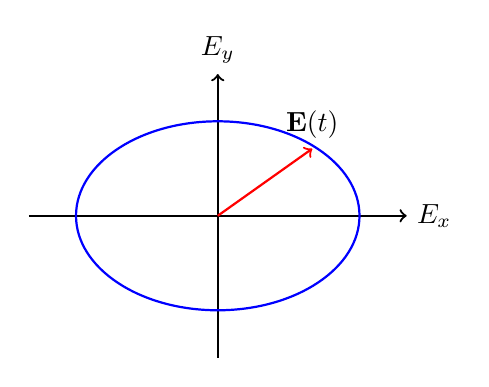
\begin{tikzpicture}[scale=1.2]
            \draw[thick,->] (-2,0) -- (2,0) node[right] {$E_x$};
            \draw[thick,->] (0,-1.5) -- (0,1.5) node[above] {$E_y$};
            \draw[thick,blue] (0,0) ellipse (1.5cm and 1cm);
            \draw[thick,->,red] (0,0) -- (1,0.71) node[at end, above, black] {$\mathbf{E}(t)$};
        \end{tikzpicture}
        \caption{Elliptical polarization}
    \end{subfigure}
    \hfill
    % Second plot: Circle
    \begin{subfigure}[b]{0.3\textwidth}
        \centering
        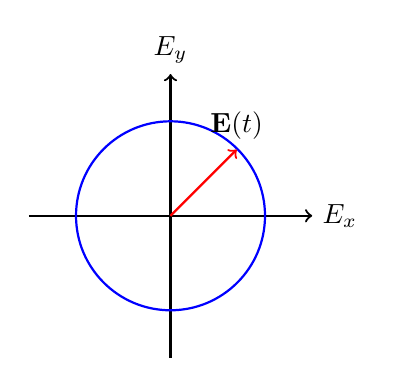
\begin{tikzpicture}[scale=1.2]
            \draw[thick,->] (-1.5,0) -- (1.5,0) node[right] {$E_x$};
            \draw[thick,->] (0,-1.5) -- (0,1.5) node[above] {$E_y$};
            \draw[thick,blue] (0,0) circle (1cm);
            \draw[thick,->,red] (0,0) -- (0.7,0.7) node[at end, above,black] {$\mathbf{E}(t)$};
        \end{tikzpicture}
        \caption{Circular polarization}
    \end{subfigure}
    \hfill
    % Third plot: Inclined line
    \begin{subfigure}[b]{0.3\textwidth}
        \centering
        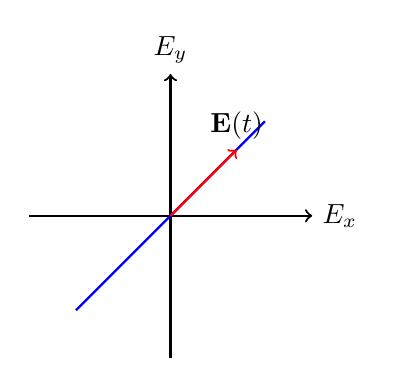
\begin{tikzpicture}[scale=1.2]
            \draw[thick,->] (-1.5,0) -- (1.5,0) node[right] {$E_x$};
            \draw[thick,->] (0,-1.5) -- (0,1.5) node[above] {$E_y$};
            \draw[thick,blue] (-1,-1) -- (1,1);
            \draw[thick,->,red] (0,0) -- (0.7,0.7) node[at end, above, black ] {$\mathbf{E}(t)$};
        \end{tikzpicture}
        \caption{Linear polarization}
    \end{subfigure}
    \caption{The plots of the electric field in the xy plane: each point of the plot corresponds to the electric field at a given time. In the first plot (a) the general elliptical polarization is represented, while in other two plots the electric field with circular (b) and linear polarization (a) are represented.}
    \label{fig:E_polarization}
\end{figure}
In general, the polarization describes how the electric field, of a wave, oscillates: indeed, figure \ref{fig:E_polarization} shows that for linear polarization, for example, the electric field oscillates in a precise direction. The polarization of a photon can be  described the \textbf{Stokes parameters}:
\begin{align}\label{eq:stokes_parameters}
    I&\defeq |E_x|^2+|E_y|^2,\qquad &Q\defeq |E_x|^2-|E_y|^2,&&\nonumber\\ U&\defeq 2|E_x||E_y|\cos\phi,\qquad &V\defeq 2|E_x||E_y|\sin\phi,&&
\end{align}
where $I$ is the intensity of the light while $Q,U$ and $V$ describe the polarization. Indeed, for linear polarized light $U=V=0$ while $Q$ is related to the direction of oscillation. On the other hand, for circular polarization $Q=U=0$ while $V\neq0$.\\Circular polarization is not produced in the early universe, therefore we will set $V=0$, so that we are describing only linearly polarized or unpolarized light.

Before proceeding, we should note that under rotations in the $xy$ plane $$E_x\rightarrow E_x\cos\theta-E_y\sin\theta,\qquad E_y\rightarrow E_x\sin\theta+E_y\cos\theta,$$ the  Stokes parameters will transform as
$$I\rightarrow I,\qquad Q\pm iU\rightarrow e^{\pm 2i\theta}(Q\pm iU).$$
This transformation shows that the combination $(Q\pm iU)$ transforms as a \emph{spin-2 tensor} while $I$ as a scalar. This observation will be crucial when will need to decompose these modes. The above transformation makes also more clear the interpretation of the parameter $U$: from the above we have $U'=\text{Im}\big[\exp(\pm2i\theta)(Q\pm iU)\big]$, thus for $\theta= \pm\pi/2$ we have $U'=\pm Q$, showing that $U$ is the difference of the components of $\mathbf{E}$ along the bisectors of the x and y axis.

Now that we know how to describe polarized light, let's move to study how \emph{Compton scattering} is influenced by polarization. Consider an electron, on which light can be scatter off, the interaction can absorb some components of the electric field, letting the other unchanged, modifying the polarization of the photon.\\
For example, an unpolarized photon moving along the $x$ axis and deflected along the $z$ axis, in the end, will have a polarization along the $y$ axis. This is due to the simple fact that $\mathbf{E}$ and $\mathbf{B}$ must be orthogonal to the direction of motion and therefore any component along the $z$ axis will be absorbed by the electron (as shown in figure \ref{fig:compton_polarization} (a)).

\begin{figure}[h]
    \centering
    \begin{subfigure}[b]{0.45\textwidth}
        \centering
        \label{fig:compton_unpol}
        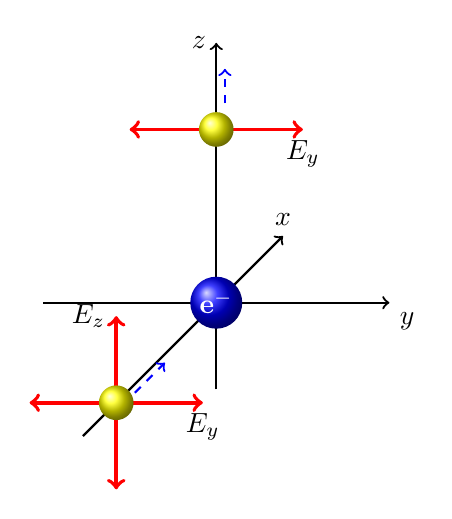
\begin{tikzpicture}[scale=1.1]
            % Draw the axes
            \draw[thick,->] (-2,0,0) -- (2,0,0) node[below right] {$y$};
            \draw[thick,->] (0,-1,0) -- (0,3,0) node[left] {$z$};
            \draw[thick,<-] (0,0,-2) node[above] {$x$}-- (0,0,4);

            % Electric field components of the photon along z-axis
            \draw[<->,red,line width=1.4pt] (-1,2,0) -- (1,2,0) node[below , black] {$E_y$};
    
            % Photon moving along the z-axis
            \draw[->,blue,thick, dashed] (0.1,2.3,0) -- (0.1,2.7,0);
            \shade[ball color=yellow] (0,2,0) circle (0.2cm);
            
        
            % Electric field components of the photon along x-axis
            \draw[<->,red,line width=1.4pt] (0,-1,3) -- (0,1,3) node[left, black] {$E_z$};
            \draw[<->,red,line width=1.4pt] (-1,0,3) -- (1,0,3) node[below , black] {$E_y$};
    
            % Photon moving along the x-axis
            \draw[->,blue,thick, dashed] (0.1,0,2.7) -- (0.1,0,1.8);
            \shade[ball color=yellow] (0,0,3) circle (0.2cm);
        
            % Electron at the origin
            \shade[ball color=blue] (0,0,0) circle (0.3cm);
            \node[thick, white] at (0,0,0) {$\mathbf{e^-}$};
        
        \end{tikzpicture}
        \caption{Unpolarized light}
    \end{subfigure}
    \begin{subfigure}[b]{0.45\textwidth}
        \centering
        \label{fig:Compton_quadrupole}
    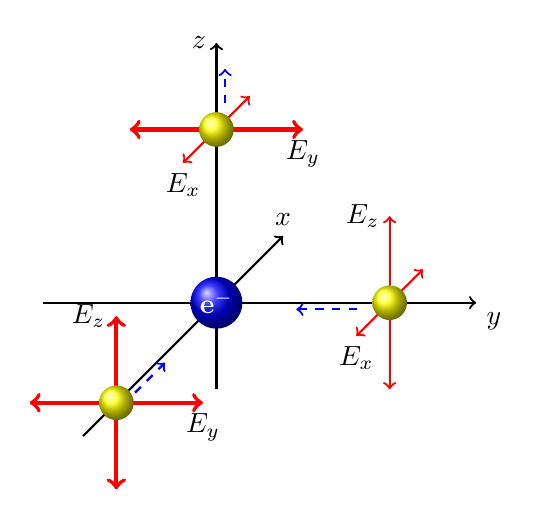
\begin{tikzpicture}[scale=1.1]
        % Draw the axes
        \draw[thick,->] (-2,0,0) -- (3,0,0) node[below right] {$y$};
        \draw[thick,->] (0,-1,0) -- (0,3,0) node[left] {$z$};
        \draw[thick,<-] (0,0,-2) node[above] {$x$}-- (0,0,4);

        % Electric field components of the photon along z-axis
        \draw[<->,red,line width=1.5pt] (-1,2,0) -- (1,2,0) node[below , black] {$E_y$};
        \draw[<->,red,thick] (0,2,-1) -- (0,2,1) node[below , black] {$E_x$};

        % Photon moving along the z-axis
        \draw[->,blue,thick, dashed] (0.1,2.3,0) -- (0.1,2.7,0);
        \shade[ball color=yellow] (0,2,0) circle (0.2cm);
        
    
        % Electric field components of the photon along x-axis
        \draw[<->,red,line width=1.5pt] (0,-1,3) -- (0,1,3) node[left, black] {$E_z$};
        \draw[<->,red,line width=1.5pt] (-1,0,3) -- (1,0,3) node[below , black] {$E_y$};

        % Photon moving along the x-axis
        \draw[->,blue,thick, dashed] (0.1,0,2.7) -- (0.1,0,1.8);
        \shade[ball color=yellow] (0,0,3) circle (0.2cm);
        
        % Electric field components of the photon along y-axis
        \draw[<->,red,thick] (2,-1,0) -- (2,1,0) node[left, black] {$E_z$};
        \draw[<->,red,thick] (2,0,-1) -- (2,0,1) node[below , black] {$E_x$};

        % Photon moving along the y-axis
        \draw[->,blue,thick, dashed] (1.7,0,0.2) -- (1,0,0.2);
        \shade[ball color=yellow] (2,0,0) circle (0.2cm);
     

        % Electron at the origin
        \shade[ball color=blue] (0,0,0) circle (0.3cm);
        \node[thick, white] at (0,0,0) {$\mathbf{e^-}$};
    
    \end{tikzpicture}
    \caption{Quadrupole momentum}
    \end{subfigure}
    \caption{Graphical depiction Compton scatterings effects on polarized light. Figure \emph{(a)} shows an unpolarized photon scattered by an electron resulting in a linearly polarized photon. Figure \emph{(b)} instead shows how the presence of a quadrupole momentum can generate polarized photons by the scatterings: thicker vectors represents more intense electric fields, thus "hotter" photons.}
    \label{fig:compton_polarization}
\end{figure}
In the general case, consider some incoming radiation with polarization $\boldsymbol{\epsilon}_i'$\footnote{$\boldsymbol{\epsilon}_i'$ are the versors onto which the $\mathbf{E}$ decomposes.} which gets scattered off by an electron. The deflected radiation will instead have a polarization $\boldsymbol{\epsilon}_i$. Without loss of generality, we can orient our coordinate axis such that the outgoing radiation is travelling along the $z$ axis and the polarization $\boldsymbol{\epsilon}_1=\versor x$ and $\boldsymbol{\epsilon}_2=\versor y$.\\
The parameter $Q$, after the scattering, can be estimated decomposing the incoming polarization on the outgoing one and then averaging over all possible incoming photons:
$$Q\propto\int d\Omega_{in} f_{\text{in}}(\versor n')\sum_{i=1}^{2}\bigg[|\boldsymbol{\epsilon}_{i}'\cdot\versor{x}|^2-|\boldsymbol{\epsilon}_{i}'\cdot\versor{y}|^2\bigg],$$
where $f_{\text{in}}$ is the phase space distribution of the incoming photons.\\
As a function of the polar incoming angles, the incoming polarization can be written as
\begin{align*}
    \boldsymbol{\epsilon}_1'(\theta',\phi') &=(\cos\theta'\cos\phi',\cos\theta'\sin\phi',-\sin\theta'),\\
    \boldsymbol{\epsilon}_2'(\theta',\phi') &=(-\sin\phi',\cos\theta',0).
\end{align*} 
Once inserted in the previous integral we find
\begin{align*}
    Q&\propto\int d\Omega_{in} f_{\text{in}}(\versor n')\bigg[\cos^2\theta'\cos^2\phi'+\sin^2\phi'-\cos^2\theta'\sin^2\phi'-\cos^2\phi'\bigg]\\&\propto\int d\Omega_{in} f_{\text{in}}(\versor n')(\sin^2\theta'\cos2\phi')\propto\int d\Omega_{\text{in}}f_{\text{in}}(\versor n')\bigg[Y_{2,2}(\versor n')+Y_{2,-2}(\versor n')\bigg],
\end{align*}
where we recognized, in the last step, that $\sin^2\phi'\cos2\phi'$ is proportional to the sum of two spherical harmonics\footnote{Recall that $Y_{\ell,\pm\ell}(\theta,\phi)=\frac{(\mp)^\ell}{2^\ell\ell!}\sqrt{\frac{(2\ell+1)!}{4\pi}}\sin^\ell\theta\ e^{\pm i\ell\phi}$ and therefore $Y_{2,2}+Y_{2,-2}\propto sin^2\theta\cos2\phi$.}.\\
Now, considering perturbations of the temperature in $f_{\text{in}}$, as in \eqref{eq:phspdist_perturb}, we discover that, since the integral picks the modes with $\ell=2$, polarization will be generated through Compton scatterings by the quadrupole momentum $\Theta_2$. Similar calculations can lead to the same conclusion for the parameter $U$.\\ Intuitively, this can be understood considering two unpolarized photons, with different energies (thus temperatures when we consider an ensemble), travelling towards an electron from orthogonal directions: this simplified setting corresponds to a quadrupole momentum of the anisotropies. Then, a photon scattered in the z direction will then have one component of its electric field given by the first photon and the other component from the second photon, as represented in figure \ref{fig:compton_polarization} (b). Since the two photons have different energies, the electric field components of the scattered photon will be different, giving a polarization to it. 

To appropriately describe polarization in the context of anisotropies we must develop a proper framework. Let's start considering linear polarized light propagating in the $z$ direction: the stokes parameter $Q$ will therefore measure the difference of the energy density (recall $\rho\propto \mathbf{E}^2$) associated to the electric field components $E_x$ and $E_y$.\\ This radiation can be seen as the superposition of two gasses of photons: each one will be made by photons described by one of the two components of the electric field. Then, each gas will have its own phase space distribution: $f_x$ and $f_y$. Note that if the two distributions are identical the light turns out to be unpolarized with respect to $Q$: indeed the two gasses would have the same temperature and thus the two components of $\mathbf{E}$ would be equal, giving $Q=0$\footnote{For now, we just consider $Q$ later on we will also find a way to describe $U$.}. Hence, we need to consider temperature anisotropies between the two distributions: to better describe these we introduce a \emph{phase space matrix}
\begin{equation}
    \label{eq:Pol_Occup_Matrix}
    \mathcal{F} _\text{unpol} \defeq
    \begin{pmatrix}
        f_x(\bar T) & 0 \\ 0 & f_y(\bar T)
    \end{pmatrix}\ \xrightarrow{\text{polarization}}\mathcal{F}  \defeq
    \begin{pmatrix}
        f_x(\bar T[1+\Theta_x]) & 0 \\ 0 & f_y(\bar T[1+\Theta_y ])
    \end{pmatrix},
\end{equation}
where $\Theta_x(x^\mu,\mathbf n)$ and $\Theta_y(x^\mu,\mathbf n)$ are the fluctuations around the mean temperature $\bar T$. The total phase space distribution is then recovered by taking the trace of the above matrices $f=\text{Tr}(\mathcal{F} )/2$, which corresponds to the average of the components.\\
From these two anisotropies we can define, recalling that $T^4\propto\rho\propto\mathbf{E}^2$,
\begin{align}
    \label{eq:ThetaQ}
    \Theta_Q&\defeq\Theta_x-\Theta_y\\&=\frac{\Delta T_x-\Delta T_y}{\bar T}=\frac{\Delta\rho_x-\Delta\rho_y}{4\bar\rho}=\frac{(E_x^2-\mathbf{E}^2)-(E_x^2-\mathbf{E}^2)}{4\mathbf{E}^2}=\frac{Q}{4I},\nonumber
\end{align}
where we used the approximation $\Delta\rho/\rho\propto4\Delta T/T$ for small perturbations.\\The same hols for $\Theta_U=U/(4I)$, since we just need to rotate the axis to turn $Q\rightarrow U$, then we can repeat the above calculations and rotate everything back.\\ Lastly, we want to describe polarization by a single parameter, this can be done exploiting rotations. Suppose we have described chosen the axis such that $Q\neq0$ and $U=0$, in this way $\Theta_Q$ describes the anisotropies related to the "amplitude" of polarization and $\Theta_U$ is not needed. To allow for a generic orientation of the axis we rotate the $xy$ plane defining the amplitude $\Theta_P$ to correspond to the previous $\Theta_Q$, which now instead reads
$$\Theta_Q=\Theta_P\cos2\phi,\qquad\text{while}\  \Theta_U=\Theta_P\sin2\phi.$$
Note that the above discussion holds only for monochromatic waves. When dealing with a Fourier decomposition these two last formulae hold only in the limit $\versor n\cdot\versor k\ll1$, with $\versor{n}$ direction of propagation of the full wave.

$\Theta_P$ will then evolve with its own Boltzmann equation:
all the physics described previously is unchanged, however we need to account for Compton scattering effect con polarization. Indeed, we already discussed that the quadrupole $\tilde{\Theta}_2$ will polarize scattered photons, therefore a collision term proportional to $\Theta_2$ must be added to the Boltzmann equation \eqref{eq:phot_boltzmann_pert}. Furthermore, if polarization is not sourced, through Compton scattering the radiation will gradually become unpolarized. This means that now a term proportional to $-\tilde{\Theta}_P$ must be added as a collision contribution. The final result, derived in \cite{10.1093/mnras/226.3.655}, is the Boltzmann equation for the polarization anisotropy:
\begin{equation}\label{eq:ThetaP_Boltzmann}
    \frac{\partial \tilde\Theta_P}{\partial t}+\frac{ik\mu}{a}\tilde\Theta_P=-n_e\sigma_T\bigg[\tilde\Theta_{P}+\frac{1}{2}\bigg(1-P_2(\mu)\bigg)\Pi\bigg],
\end{equation}
where $\Pi=\tilde\Theta_2+\tilde\Theta_{P,2}+\tilde\Theta_{P,0}$ and $P_2(\mu)=\frac{3\mu^2-1}{2}$ is the order 2 Legendre polynomial.
Then, polarization will affect also the regular collision term for Compton scattering, hence equation \eqref{eq:phot_boltzmann_pert} must be corrected:
\begin{equation}\label{eq:phot_boltzmann_pert_pol}
    \frac{\partial \tilde\Theta}{\partial t} +\frac{ik\mu}{a}\tilde\Theta+\frac{\partial \tilde\Psi}{\partial t}+\frac{ik\mu}{a}\tilde\Phi=n_e \sigma_T\Bigg[\tilde\Theta_0-\tilde\Theta-i\mu\tilde v_b-\frac{1}{4}P_2(\mu)\Pi\Bigg].
\end{equation}
\subsection{Multipole expansion of the Boltzmann equation}\label{sec:BoltzmannMultipoleExpansion}
In section \ref{sec:ComptonPolarization} we obtained the differential equations \eqref{eq:phot_boltzmann_pert_pol} and \eqref{eq:ThetaP_Boltzmann} governing the time evolution of the anisotropies in the CMB. To end our discussion of the time evolution of the anisotropies we want to expand these equations in multipoles.

Since the CMB is observed in the sky, spherical harmonics are the natural basis to use to project the anisotropies. The fact that the equations \eqref{eq:phot_boltzmann_pert_pol} and \eqref{eq:ThetaP_Boltzmann} depend only on $\mu=\versor p\cdot\versor k$, corresponds to a rotational symmetry of the system around one of these two vectors. By using spherical polar coordinates, such that the vector $\versor k$ lies on the $z$ axis, the above symmetry corresponds to a rotational symmetry of the azimuthal angle $\phi$. Considering that $Y_{\ell m}\propto e^{im\phi}$, we immediately recognize that such symmetry is respected only by spherical harmonics with $m=0$ and these precisely corresponds to the Legendre polynomials. Therefore, for scalar perturbation, we can limit ourselves to a multipole expansion on the Legendre polynomials, without worrying of all the spherical harmonics.

By multiplying the \eqref{eq:phot_boltzmann_pert_pol} by the order $\ell$ Legendre polynomial $P_\ell(\mu)\times i^\ell/2$ and integrating over $\mu$, we can exploit the orthogonality of the Legendre polynomials as follows.
\begin{itemize}
    \item $\frac{\partial \tilde\Theta}{\partial t} $ and $n_e\sigma_T\tilde{\Theta}$ depending on $\mu$ in this expansion will give contributions corresponding respectively to $\frac{\partial \tilde\Theta_\ell}{\partial t} $ and $n_e\sigma_T\tilde{\Theta}_\ell$ (from the expansion definition \eqref{eq:legendre_expansion}).
    \item $\frac{\partial\tilde\Psi}{\partial t}$ and $n_e\sigma_T\tilde\Theta_0$ have no $\mu$ dependence, which corresponds to the zeroth order Legendre polynomial $P_0(\mu)=1$, and thus they only contribute to the $\ell=0$ equation.
    \item $\tilde\Phi$ and $n_e\sigma_T\tilde v_b$ are multiplied by $P_1(\mu)=\mu$, giving contributions only to $\ell=1$ equation, while $\Pi$ is multiplied by $P_2(\mu)=\frac{3\mu^2-1}{2}$, contributing only to $\ell=2$ equation. Note that these terms must also be multiplied by a factor corresponding to the integral of their respective Legendre polynomial squared, since they don't contain any $\tilde\Theta$ function to be expanded.
    \item $\frac{ik\mu}{a}\tilde\Theta$ is instead more complicated since it is the product of two functions depending on $\mu$. Bonnet's formula \eqref{eq:bonnet} allows us to simplify the corresponding integral 
    $$\frac{i^\ell}{2}\int_{-1}^{+1}d\mu\ \mu P_\ell(\mu)\tilde\Theta=\frac{i^\ell}{2}\int_{-1}^{+1}d\mu \bigg[\frac{\ell+1}{2\ell+1}P_{\ell+1}(\mu)+\frac{\ell}{2\ell+1}P_{\ell-1}(\mu)\bigg]\tilde\Theta,$$
    in this way this will give contributions to all the equations coupling them together.
\end{itemize}
Putting all of this together we obtain the following coupled system of differential equations
\begin{subequations}\label{eq:multipole_boltzmann_photons}
    \begin{align}
           &\dot{\tilde{\Theta}}_0=-\frac{k}{a}\tilde{\Theta}_1-\dot{\tilde\Psi}\label{eq:multipole_boltzmann_photons_0}\\
            &\dot{\tilde{\Theta}}_1=\frac{k}{3a}\tilde\Theta_0-\frac{2k}{3a}\tilde\Theta_2+\frac{k}{3}\tilde\Phi-n_e\sigma_T\bigg[\tilde\Theta_1-\frac{\tilde v_b}{3}\bigg]\label{eq:multipole_boltzmann_photons_2}\\
            &\dot{\tilde{\Theta}}_\ell=\frac{\ell k}{(2\ell+1)a}\tilde\Theta_{\ell-1}-\frac{(\ell+1)k}{(2\ell+1)a}\tilde\Theta_{\ell+1}-n_e\sigma_T\bigg[\tilde\Theta_\ell-\frac{\delta_{\ell,2}}{10}\Pi\bigg]\qquad \ell\geq 2,\label{eq:multipole_boltzmann_photons_3}
        \end{align}
\end{subequations}

Similarly, equation \eqref{eq:ThetaP_Boltzmann} will result in the following system of differential equations
\begin{subequations}\label{eq:multipole_boltzmann_polatization}
    \begin{align}
           &\dot{\tilde{\Theta}}_{P,0}=-\frac{k}{a}\tilde{\Theta}_{P,1}-n_e\sigma_T\bigg[\tilde\Theta_{P,0}-\frac{1}{2}\Pi\bigg]\label{eq:multipole_boltzmann_polatization_0}\\
            &\dot{\tilde{\Theta}}_{P,\ell}=\frac{\ell k}{(2\ell+1)a}\tilde\Theta_{P,\ell-1}-\frac{(\ell+1)k}{(2\ell+1)a}\tilde\Theta_{P,\ell+1}-n_e\sigma_T\bigg[\tilde\Theta_{P,\ell}-\frac{\delta_{\ell,2}}{10}\Pi\bigg]\qquad \ell\geq 1,\label{eq:multipole_boltzmann_polatization_2}.
        \end{align}
\end{subequations}  
Equations \eqref{eq:multipole_boltzmann_photons} and \eqref{eq:multipole_boltzmann_polatization} are not the full system of coupled equations, indeed these equations depend on the potential $\tilde\Psi$ and $\tilde\Phi$ and on the electron bulk velocity $\tilde v_b$. The differential equations governing these quantities must then be added to the ones above and solved all together.\\
Note that, in the above equations, $\Psi$ and $\Phi$ appears only in the equation with $\ell=0,1$: this means that primordial perturbations source directly only the first two momenta of the anisotropies. Then, since all the equations are coupled together, the dynamics of the anisotropies will give rise to the other momenta.
\subsection{Polarization anisotropies power spectrum}\label{sec:PolarizationPowerSpectrum}
We already discussed that, in order to completely describe photons (thus the CMB), we also need to account for polarization. It is therefore natural to define a power spectrum for the polarization anisotropies, which can be done similarly as for the temperature.

We want to expand onto the sky (really the dependence from the direction of observation $\versor n$) $\Theta_Q$ and $\Theta_UU$, however we showed, in section \ref{sec:ComptonPolarization} that under a rotation the combination $Q\pm iU$ (and thus their respective $\Theta$s) will transform as a spin 2 fields. This means that we cannot resort to the usual spherical harmonics decomposition, instead we must use \textbf{spin-weighted spherical harmonics} $Y_{\ell m}^{\pm2}$. In Fourier space such expansion reads. This expansion reads   
\begin{equation}
    (\Theta_Q\pm i\Theta_U)(\versor n)=\sum_{\ell m} Y^{\pm2}_{\ell m}(\versor n)a^{\pm2}_{\ell m} ,\label{eq:EB_sky_expansion}
\end{equation}
The coefficients we obtained can be then combined into parity even or odd combinations that turns out to be the multipoles of the so called \textbf{E-modes} and \textbf{B-modes}:
\begin{align*}
    a^E_{\ell m}&\defeq-\frac{a^2_{\ell m}+a^{-2}_{\ell m}}{2},\qquad &E(\versor n)=\sum_{\ell m}a^E_{\ell m}Y_{\ell m}(\versor n),&&\\ a^B_{\ell m}&\defeq\frac{a^2_{\ell m}-a^{-2}_{\ell m}}{2i}
    \qquad &B(\versor n)=\sum_{\ell m}a^B_{\ell m}Y_{\ell m}(\versor n).&&
\end{align*}
The power spectra of the polarization can then be defined, as usual, as
\begin{align}\label{eq:PolPowerSpectrum}
    \langle a^E_{\ell m}a^{E*}_{\ell' m'}\rangle\defeq C_{\ell}^{EE}\delta_{\ell \ell'}\delta_{m m'},\\ \langle a^B_{\ell m}a^{B*}_{\ell' m'}\rangle\defeq C_{\ell}^{BB}\delta_{\ell \ell'}\delta_{m m'},\\\langle a_{\ell m}a^{E*}_{\ell' m'}\rangle\defeq C_{\ell}^{TE}\delta_{\ell \ell'}\delta_{m m'}.
\end{align}
\section{Tensor perturbations effects on the CMB}\label{sec:Anisotropies_From_Tensor}
In the previous sections we focused on how the scalar perturbations interact with the CMB generating anisotropies. We will instead now study how tensor perturbations, namely gravitational waves produced during inflation, affects the evolution of the plasma of photons and what kind of anisotropies are sourced by them.

In appendix \ref{app:tensorPerturbedLiouvilleOperator} we showed that, considering tensor perturbed metric $$ds^2=-dt^2+a^2(\delta_{ij}h_{ij})dx^dx^j,$$the \emph{Liouville operator} reads as in \eqref{eq:tensorPerturbedLiouvilleOperator}
$$\hat{\mathbf{L}}[f]=\frac{\partial f}{\partial t}+\frac{\hat p^i}{a}\frac{\partial f}{\partial x^i}-\frac{1}{2}\frac{\partial f}{\partial t}\dot{h}_{ij}\hat p^i\hat p^j+\text{second order terms},$$
where $p^i=p\ \hat p^i$ is the local 3-momentum of a photon and $f$ the phase space distribution.

To obtain the equation describing the evolution of anisotropies, we must expand the photon phase space distribution on a blackbody radiation background ($\bar{f}(t,p)+\Upsilon(x^\mu,\mathbf p) $) and assume that the temperature is perturbed as $T(x^\mu,\versor p)=\bar T (1+\Theta(x^\mu,\versor{p}))$. Proceeding in the same way as in section \ref{sec:ThetaTimeEvolution} with the above Liouville operator, we obtain the Liouville operator for the distribution perturbation 
$$\hat{\mathbf{L}}[\Upsilon]=-p\frac{\partial \bar f}{\partial p}\bigg[\frac{\partial \Theta}{\partial t}+\frac{\hat p^i}{a}\frac{\partial \Theta}{\partial x^i}+\frac{1}{2}\dot{h}_{ij}\hat p^i\hat p^j\bigg].$$
At this point we need to add the first order collision term associated to Compton scattering. For now let's consider the simplified form \eqref{eq:first_collision_term}. Using Boltzmann equation and canceling out the common factor $-p\frac{\partial\bar f}{\partial t}$ from both sides, as in section \ref{sec:ThetaTimeEvolution}, we get the differential equation that describes the time evolution of the CMB anisotropies in presence of tensor perturbations
\begin{equation}
    \label{eq:tensor_anisotropies_boltzmann}
    \frac{\partial \Theta}{\partial t}+\frac{\hat p^i}{a}\frac{\partial \Theta}{\partial x^i}+\frac{1}{2}\dot{h}_{ij}\hat p^i\hat p^j=n_{e}\sigma_T\bigg[\Theta_0-\Theta+\mathbf{\hat{p}}\cdot\mathbf{v}_{b}\bigg].
\end{equation}
Again, note that the tensor perturbations can be a source for the anisotropies, as for the scalar case.
\subsection{Coupling of tensors pertubations to anisotropies}\label{sec:TensorCoupling}
Previously, to expand equation \eqref{eq:phot_boltzmann_pert}, we Fourier transformed $\Theta(t,\mathbf{x},\versor p)$ and then expanded it in Legendre polynomials. However, this last step was justified (in section \ref{sec:BoltzmannMultipoleExpansion}) by noting that the equations depended only on the cosine of angle between the direction of motion of the photon $\versor p$ and the wave number vector of the Fourier transform $\mathbf{k}$. This corresponded to a rotational symmetry around one of the above vectors that implied that Legendre polynomials were the appropriate basis to expand on. We shall now study equation \eqref{eq:tensor_anisotropies_boltzmann}, and its symmetries, to understand  what will now be the right basis to use for this expansion.

To begin, let's recall that, being traceless transverse, in Fourier space $h_{ij}$ can be separated in two independent polarizations
\begin{align*}
    0=\partial^ih_{ij}=\int\frac{d^3k}{(2\pi)^3}e^{\mathbf{k}\cdot\mathbf{x}}\tilde h_{ij}k^i \ \xrightarrow{\substack{\text{Traceless}\\\text{Symmetric}}}\ \tilde h_{ij}=\tilde h_{\boldsymbol \times} \mathbf{e}_{ij}^{\boldsymbol \times}+\tilde h_{\boldsymbol +} \mathbf{e}_{ij}^{\boldsymbol +}=
    \begin{pmatrix}
        \tilde h_{\boldsymbol \times} & \tilde h_{\boldsymbol +} & 0\\
        \tilde h_{\boldsymbol +} & -\tilde h_{\boldsymbol \times} & 0\\
        0&0&0
    \end{pmatrix}.
\end{align*}
Now, the only term in equation \eqref{eq:tensor_anisotropies_boltzmann} that could give a more complicated angular dependence (that just $\cos\theta$) is $\dot{h}_{ij}\hat p^i\hat p^j$: considering spherical polar coordinates $(r,\theta,\phi)$ with $\mathbf k\parallel \versor z$, once Fourier transformed, this term will be proportional to
\begin{align*}
    \versor p=(\sin\theta\cos\phi,\sin\theta\sin\phi,\cos\theta)\quad \Rightarrow\quad (\mathbf{e}_{ij}^{\boldsymbol \times}+\mathbf{e}_{ij}^{\boldsymbol +})\hat p^i\hat p^j=\sin^2\theta(\cos2\phi+\sin2\phi).
\end{align*} 
This clearly shows that anisotropies coupled to tensor perturbations can no longer be decomposed on Legendre polynomials, since the azimuthal symmetry is now spoiled by the explicit dependence on $\phi$.

To individuate the appropriate basis for the spherical harmonics expansion, let's use the basis introduced by Hu and White in \cite{HuWhite}
\begin{equation}
    \label{eq:HuWhiteBasis}
    h_{ij}=-\sqrt{\frac{3}{2}}(h^{(+)}\mathbf{e}_{ij}^{(+)}+h^{(-)}\mathbf{e}_{ij}^{(-)}) \quad \text{with } \mathbf{e}^{(+)}=\begin{pmatrix}
        1&+i&0\\+i&-1&0\\0&0&0
    \end{pmatrix}\ \mathbf{e}^{(-)}=\begin{pmatrix}
        1&-i&0\\-i&-1&0\\0&0&0
    \end{pmatrix}.
\end{equation}
Comparing this definition and the previous basis, we can easily find the transformation between the two polarizations
\begin{align*}
    h_{\boldsymbol{+}}&=-\sqrt\frac{3}{2}(h^{(+)}+h^{(-)}),\qquad &h^{(+)}&=\frac{1}{\sqrt{6}}(h_{\boldsymbol{+}}-ih_{\boldsymbol{-}}),\\ h_{\boldsymbol{+}}&=-i\sqrt\frac{3}{2}(h^{(+)}-h^{(-)}),\qquad &h^{(-)}&=-\frac{1}{\sqrt{6}}(h_{\boldsymbol{+}}+ih_{\boldsymbol{-}}).
\end{align*}
Let's now project the versor $\versor p$, defined as above, onto $\mathbf{e}^{(\pm)}$, 
$$\mathbf{e}_{ij}^{(\pm)}\hat p^i\hat p^j=\sin^2\theta[\cos^2\phi-\sin^2\phi\pm2i\sin\phi\cos\phi]=\sin^2\theta e^{\pm i2\phi},$$
immediately we should recognize that this term is proportional to the spherical harmonics $Y_{2,\pm2}(\theta,\phi)=\frac{1}{4} \sqrt{\frac{15}{2\pi}} \, \sin^2\theta \, e^{ \pm i2\phi}$. This shows that the appropriate basis for the expansion of the anisotropies are the spherical harmonics $Y_{\ell m}$ with $m=\pm2$, since they all posses the same azimuthal symmetry $Y_{\ell m} \propto e^{\pm i2\phi}$ as the tensor term in \eqref{eq:tensor_anisotropies_boltzmann}.

Following Hu and White \cite{HuWhite} convention, we will use the following multipole expansion for the anisotropies
\begin{equation}
    \label{eq:TensorMultipoleExpansion}
    \Theta(t,\mathbf x,\versor p)=\int\frac{d^3k}{(2\pi)^3}e^{i\mathbf{k}\cdot\mathbf{x}}\sum_{\ell m} (-i)^{\ell}\sqrt{\frac{4\pi}{2\ell+1}}Y_{\ell m}(\versor p)\tilde\Theta_{\ell}^{(m)}(t,\mathbf k) ,
\end{equation}
in which we will only use the multipoles with $m=\pm2$, for the reasons we just explained.\\ Note that for $m=0$, since $Y_{\ell 0}=\sqrt{\frac{2\ell+1}{4\pi}}P_\ell(\cos\theta)$, we recover the Legendre polynomials expansion used for scalar perturbations. In this case the sum over the $2\ell+1$ different values of $m$ will result in the correspondence $\tilde \Theta_\ell^{(0)}=(2\ell+1)\tilde\Theta_{\ell}$.\\Lastly, we shall note that the normalization of the new polarization \eqref{eq:HuWhiteBasis} is such that 
\begin{align*}
    \frac{1}{2}\dot{\tilde{h}}_{ij}\hat p^i\hat p^j&=\frac{1}{2}\bigg(-\sqrt{\frac{3}{2}}\bigg)\bigg[\dot{\tilde{h}}^{(+)}\sin^2\theta e^{i2\phi}+\dot{\tilde{h}}^{(-)}\sin^2\theta e^{-i2\phi}\bigg]\\&=-\sqrt{\frac{4\pi}{5}}\bigg[\dot{\tilde{h}}^{(+)}Y_{2,2}(\versor p)+\dot{\tilde{h}}^{(-)}Y_{2,-2}(\versor p)\bigg],\\
\end{align*}
where the factor $-\sqrt{\frac{4\pi}{5}}$ precisely corresponds to $i^\ell\sqrt\frac{4\pi}{2\ell+1}|_{\ell=2}$, which is also the factor that get all the others $\tilde\Theta_2^{(2)}$ in the expansion. In this way the contribution of the tensor perturbation to the multipole expansion of equation \eqref{eq:tensor_anisotropies_boltzmann}, with $\ell=2$ and $m=\pm2$, will be exactly $\dot{\tilde{h}}^{(\pm)}$.
\subsection{Multipole expansion of tensor induced anisotropies}
Knowing that tensor perturbations are projected in the sky onto spherical harmonics with $m=\pm2$ while scalar perturbations are projected onto spherical harmonics with $m=0$, by their orthogonality, we can expand $\Theta$ in multipoles using only $Y_{\ell,\pm2}$. In this way we effectively decoupled the multipoles generated by tensor perturbations and the scalar ones.

First, we move to Fourier space where the equation describing anisotropies \eqref{eq:tensor_anisotropies_boltzmann} reads
$$\frac{\partial\tilde \Theta}{\partial t}+i\frac{k\cos\theta}{a} \tilde\Theta-\sqrt{\frac{4\pi}{5}}\bigg[\dot{\tilde{h}}^{(+)}Y_{2,2}(\versor p)+\dot{\tilde{h}}^{(-)}Y_{2,-2}(\versor p)\bigg]=n_{e}\sigma_T\bigg[\tilde\Theta_0-\tilde\Theta+k\tilde v_{b}\cos\theta\bigg],$$ in which we assumed that $\mathbf{v}_b$ is irrotational. \\Now, the expansion in spherical harmonics \eqref{eq:TensorMultipoleExpansion} yields 
$$\tilde{\Theta}_{\ell}^{(m)}(\mathbf{k})=i^\ell\sqrt{\frac{2\ell+1}{4\pi}}\int d\Omega_{\versor p}\tilde\Theta(\mathbf{x},\versor p)Y_{\ell,m}^*(\theta,\phi),$$
therefore, upon integration of the equation above we can decompose it in a set of ordinary differential equations, one for each multipole $\Theta_\ell^{(m)}$.\\
However, similarly to what happened in section \ref{sec:BoltzmannMultipoleExpansion}, we obtain from the second term on the left-hand side a contribution proportional to $Y^*_{\ell m}(\theta,\phi)\cos\theta$. The proprieties of spherical harmonics allows to simplify this term as follows
$$
\cos\theta Y_{\ell m}(\theta,\phi)=\sqrt\frac{4\pi}{3}Y_{10}Y_{\ell m}=\sqrt{\frac{\ell^2-m^2}{(2\ell-1)(2\ell+1)}}Y_{\ell-1,m}+\sqrt{\frac{(\ell+1)^2-m^2}{(2\ell+3)(2\ell+1)}}Y_{\ell+1,m}
$$  and upon integration we therefore also get contributions from other multipoles.\\In this way equation \eqref{eq:tensor_anisotropies_boltzmann}
will be decomposed into
\begin{subequations}
    \begin{align}
    \dot{\tilde\Theta}_2^{(\pm2)}&=-\frac{\sqrt{5}}{7a}k\tilde\Theta_3^{(\pm2)}-n_e\sigma_T\tilde\Theta_{2}^{(\pm2)}-\dot{\tilde h}^{(\pm)}\quad \\
    \dot{\tilde\Theta}_\ell^{(\pm2)}&=\frac{k}{a}\bigg[\frac{\sqrt{\ell^2-4}}{2\ell-1}\tilde\Theta_{\ell-1}^{(\pm2)}-\frac{\sqrt{(\ell+1)^2-4}}{2\ell+3}\tilde\Theta_{\ell+1}^{(\pm2)}\bigg]-n_e\sigma_T\tilde\Theta_{\ell}^{(\pm2)}\quad \ell\geq3,
\end{align}
\end{subequations}

where the contributions from $\tilde{\Theta_0}$ and $\tilde v_b$ are not appearing since they are multiplied by the $m=0$ spherical harmonics. Note that this time the primordial perturbations directly source a quadrupole momentum, that then can source the higher momenta.

As we discussed in section \ref{sec:ComptonPolarization} the Compton scattering is influenced by the polarization of incoming and outgoing photons. For this reason we must add corrections to the above equations, to do so we must first describe the dynamics of the polarization.\\ The proper expansion to decouple the Boltzmann equation is a similar expansion we used in section \ref{sec:PolarizationPowerSpectrum}: in Fourier space we will follow the convention of Chluba \cite{Chluba_tens_diss}, to be consistent with the previous expansions,
\begin{equation*}
    (\Theta_Q\pm i\Theta_U)(\mathbf{x,\versor p})=\int\frac{d^3k}{(2\pi)^3}e^{i\mathbf{k}\cdot\mathbf{x}}\sum_{\ell m} (-i)^{\ell}\sqrt{\frac{4\pi}{2\ell+1}}Y^{\pm2}_{\ell m}(\versor p)(\tilde E_{\ell}^{(m)}\pm i\tilde B_\ell^{(m)}),
\end{equation*}
where $Y^{\pm2}_{\ell m}$ are again the \emph{spin weighted spherical harmonics}. We already discussed that, while the free streaming of photons is not influenced by the polarization, the quadrupole of the anisotropies sources polarized light and then, when not produced, at equilibrium we should obtain unpolarized light. This means that the equation for the dynamics of polarization anisotropies should be similar\footnote{The numerical factors will change due to the different relations between spin-weighted spherical harmonics and the regular ones. A comprehensive guide to these functions can be found in the first part of \cite{HuWhite}.} to the regular $\tilde\Theta^{(\pm2)}$ plus source terms for $\tilde\Theta_2$ and $-\tilde E_{\ell}^{(\pm2)},\ -\tilde B_{\ell}^{(\pm2)}$. The full derivation of these equations has been done by Hu and White in \cite{HuWhite}; the final result reads
\begin{subequations}\label{eq:EB_multipole_equations_tensor}
    \begin{align}
        \dot{\tilde E}_\ell^{(\pm2)}&=\frac{k}{a}\bigg[\frac{\ell^2-4}{\ell(2\ell-1)}\tilde E_{\ell-1}^{(\pm2)}-\frac{\pm4}{\ell(\ell+1)}\tilde B_\ell^{(\pm2)}-\frac{(\ell+1)^2-4}{(\ell+1)(2\ell+3)}\tilde E_{\ell+1}^{(\pm2)}\bigg]+\nonumber\\&\qquad\qquad\qquad\qquad\qquad\qquad\qquad\qquad\quad-n_e\sigma_T\bigg[\tilde E_{\ell}^{(\pm2)}+\sqrt{6}\Pi^{(\pm2)}\delta_{\ell,2}\bigg],\label{eq:E_multipole_equation_tensor}\\
        \dot{\tilde B}_\ell^{(\pm2)}&=\frac{k}{a}\bigg[\frac{\ell^2-4}{\ell(2\ell-1)}\tilde B_{\ell-1}^{(\pm2)}-\frac{\pm4}{\ell(\ell+1)}\tilde E_\ell^{(\pm2)}+\frac{(\ell+1)^2-4}{(\ell+1)(2\ell+3)}\tilde B_{\ell+1}^{(\pm2)}\bigg]+\nonumber\\&\qquad\qquad\qquad\qquad\qquad\qquad\qquad\qquad\qquad\qquad\qquad\quad-n_e\sigma_T\tilde B_{\ell}^{(\pm2)},\label{eq:B_multipole_equation_tensor}\\
        \nonumber &\text{with}\quad\Pi^{(\pm2)}=\frac{1}{10}\bigg[\tilde\Theta_2^{(\pm2)}-\sqrt{6}\tilde E_2^{(\pm2)}\bigg].
    \end{align}
\end{subequations}
In a similar way, also the equations for the anisotropies must be corrected, giving
\begin{subequations}\label{eq:Theta_multipole_equation_tensor}
    \begin{align}\label{eq:Theta_multipole_equation_tensor_l=2}
    \dot{\tilde\Theta}_2^{(\pm2)}&=-\frac{\sqrt{5}}{7a}k\tilde\Theta_3^{(\pm2)}+n_e\sigma_T\bigg[\Pi^{(\pm2)}-\tilde\Theta_{2}^{(\pm2)}\bigg]-\dot{\tilde h}^{(\pm)},\\\label{eq:Theta_multipole_equation_tensor_l>2}
    \dot{\tilde\Theta}_\ell^{(\pm2)}&=\frac{k}{a}\bigg[\frac{\sqrt{\ell^2-4}}{2\ell-1}\tilde\Theta_{\ell-1}^{(\pm2)}-\frac{\sqrt{(\ell+1)^2-4}}{2\ell+3}\tilde\Theta_{\ell+1}^{(\pm2)}\bigg]-n_e\sigma_T\tilde\Theta_{\ell}^{(\pm2)}\quad \ell\geq3.
\end{align}
\end{subequations}
\

Let's stop for a second to appreciate that the equations \eqref{eq:Theta_multipole_equation_tensor}, \eqref{eq:E_multipole_equation_tensor} and \eqref{eq:B_multipole_equation_tensor} do not mix the $\pm2$ modes. Furthermore, for both values of $m$ the equations read the same, this means that from now on we can study only the $m=2$ modes and then use the results to obtain the $m=-2$ ones.
\section{Approximate solutions for the dynamics of the anisotropies}\label{sec:CMBApproximations}
All the differential equations we derived are pretty hare to solve analytically, since they are strongly coupled and in theory they are an infinite number (as much as the number of multipoles). Usually we resort to numerical methods to obtain exact results, however some approximations can be useful to understand the general behavior of the CMB or even to simplify some numerical calculations.
\subsection{The tight coupling approximation}
\label{sec:TightCouplingApproximation}
At early times, when the plasma was denser and hotter, the mean free path of photons was very small and the rate of Compton scattering was very high. We will show that in this regime only the first two multipoles are  relevant to describe fully the plasma. In this limit the anisotropies behave similarly to a fluid that can be fully described by just two parameters: its density and velocity field.

The guiding idea behind the tight coupling approximations is that the scatterings between baryons and photons, in this limit, is the only relevant interaction that determines the dynamics of the anisotropies. This is equivalent to consider the limit in which $n_e\sigma_T\gg1$, which means that the mean free path ($\propto\frac{1}{n_e\sigma_T}$) is very small. Starting from scalar perturbations, in equation \eqref{eq:multipole_boltzmann_photons_3} we can drop the time derivative, since it is negligible with respect to the terms multiplied by $n_e\sigma_T$. In this way we are left with
$$\frac{\ell k}{(2\ell+1)a}\tilde\Theta_{\ell-1}-n_e\sigma_T\bigg[\tilde\Theta_\ell-\frac{\delta_{\ell,2}}{10}\Pi\bigg]=-\frac{(\ell+1)k}{(2\ell+1)a}\tilde\Theta_{\ell+1},$$
from which we can note that the term $\tilde\Theta_{\ell+1}$ is small compared to $\tilde\Theta_{\ell-1}$. This essentially prove that only the first few moments are relevant while higher multipoles are always smaller and smaller as $\ell$ increases. In this limit, we can neglect all the multipoles with $\ell\geq2$, we are thus left only with two only differential equations to be solved: equation \eqref{eq:multipole_boltzmann_photons_0} and equation \eqref{eq:multipole_boltzmann_photons_2} removing all $\Theta_\ell$ with $\ell\geq2$ (still coupled to the rest of the plasma). Similar considerations are valid for the polarization equations \eqref{eq:multipole_boltzmann_polatization_0} and \eqref{eq:multipole_boltzmann_polatization_2}, which can be simplified in the same way.

Also for tensor perturbations the tight coupling limit significantly simplifies the equations of motion. Reasoning as we have just done, from equations \eqref{eq:Theta_multipole_equation_tensor} and \eqref{eq:EB_multipole_equations_tensor} we conclude that only the multipoles with $\ell=2$ are relevant. In this way, after having dropped the time derivatives, we are left with 
$$n_e\sigma_T\bigg[\frac{1}{10}\Pi^{(\pm2)}-\tilde\Theta_2^{(\pm2)}\bigg]\approx\dot{\tilde h}^{(\pm2)},\quad\tilde E_2^{(\pm2)}\approx-\sqrt{6}\Pi^{(\pm2)},\quad\tilde B_{2}^{(\pm2)}\approx0,$$
that using the definition of $\Pi^{(\pm2)}=\frac{1}{10}[\tilde\Theta_{2}^{(\pm2)}-\sqrt 6 \tilde E_{2}^{(\pm2)}]$ gives
\begin{equation}
    \label{eq:TightCouplingTensor}
    \tilde\Theta_2^{(\pm2)}\approx-\frac{4\dot{\tilde h}^{(\pm2)}}{3n_e\sigma_T},\qquad\tilde E_2^{(\pm2)}\approx-\frac{\sqrt{6}}{4}\tilde\Theta_2^{(\pm2)},\qquad\tilde B_{2}^{(\pm2)}\approx0.
\end{equation}
This approximation will be particularly useful in the next chapter to study the spectral distortions associated to the dissipation of gravitational waves.
\subsection{Improved tight coupling approximation}
To conclude we want to present a simple way to improve the tight coupling approximation relaxing the approximation of stationary solutions, without spoiling the reduced number of multipoles excited. For the purpose of this work, we are going to focus primarily on tensor perturbations as illustrated in \cite{Chluba_tens_diss}.
Consider equations \eqref{eq:Theta_multipole_equation_tensor}, \eqref{eq:E_multipole_equation_tensor} and \eqref{eq:B_multipole_equation_tensor} with conformal time: working in tight coupling approximation we can neglect every multipole except for the quadrupoles. In this way we get
\begin{align*}
    \partial_{\tau}\tilde\Theta_{2}^{(\pm2)}&=n_e\sigma_T a\bigg[\frac{9}{10} \tilde\Theta_{2}^{(\pm2)}+\frac{\sqrt{6}}{10}\tilde E_{2}^{(\pm2)}\bigg]-\partial_{\tau}\tilde h^{(\pm)},\\
    \partial_{\tau}\tilde E_{2}^{(\pm2)}&=n_e\sigma_T a\bigg[\frac{2}{5} \tilde E_{2}^{(\pm2)}+\frac{\sqrt{6}}{10}\tilde \Theta_{2}^{(\pm2)}\bigg]-k\frac{2}{3}\tilde B_2^{\pm2},\\
    \partial_{\tau}\tilde B_{2}^{(\pm2)}&=n_e\sigma_T a\tilde B_{2}^{(\pm2)}+k\frac{2}{3}\tilde E_2^{\pm2}.
\end{align*}
To solve these equations we should proceed with an ansatz: assume that the solution has the form $ \tilde\Theta_{2}^{(2)}=A_\Theta e^{ik\tau}$, $\tilde E_{2}^{(2)}=A_E e^{ik\tau}$ and $\tilde B_{2}^{(2)}=A_B e^{ik\tau}$ and that the gravitational perturbation is $\tilde h^{(\pm)}=A_he^{ik\tau}$, where we dropped the $\pm$ since the equations are the same for both cases.\\ In this way the above system of differential equations reduces to a system of linear equations for the coefficients
\begin{align*}
    ikA_\Theta&=n_e\sigma_T a\bigg[\frac{9}{10} A_\Theta+\frac{\sqrt{6}}{10}A_E\bigg]-ik A_h,\\
    ikA_E&=n_e\sigma_T a\bigg[\frac{2}{5} A_E+\frac{\sqrt{6}}{10}A_\Theta\bigg]-k\frac{2}{3}A_B,\\
    ikA_B&=n_e\sigma_T a A_B+k\frac{2}{3}A_E.
\end{align*}
Once solved this system we find, defining $\xi\defeq\frac{k}{n_e\sigma_T a}$,
\begin{subequations}\label{eq:improved_TightCouplingApproximation}
    \begin{align}
        \frac{|A_\Theta|}{\frac{4}{3}\frac{|A_h|}{n_e\sigma_T a}}&=\sqrt\frac{1+\frac{341}{36}\xi^2+\frac{625}{324}\xi^4}{1+\frac{142}{9}\xi^2+\frac{1649}{82}\xi^4+\frac{2500}{729}\xi^6},\nonumber\\\tan\phi_\Theta&=-\frac{11}{6}\xi\frac{1+\frac{697}{99}\xi^2+\frac{1250}{891}\xi^4}{1+\frac{197}{18}\xi^2+\frac{125}{54}\xi^4},\\
        \frac{|A_E|}{\frac{4}{3}\frac{|A_h|}{n_e\sigma_T a}}&=\frac{\sqrt 6}{4}\sqrt\frac{1+\xi^2}{1+\frac{142}{9}\xi^2+\frac{1649}{82}\xi^4+\frac{2500}{729}\xi^6},\nonumber\\\tan(\phi_E-\pi)&=-\frac{13}{3}\xi\frac{1+\frac{121}{117}\xi^2}{1-\xi^2-\frac{50}{27}\xi^4},\\
        \frac{|A_B|}{\frac{4}{3}\frac{|A_h|}{n_e\sigma_T a}}&=\frac{\xi}{\sqrt 6}\sqrt\frac{1}{1+\frac{142}{9}\xi^2+\frac{1649}{82}\xi^4+\frac{2500}{729}\xi^6}\nonumber\\\tan(\phi_B-\pi)&=-\frac{16}{3}\xi\frac{1+\frac{121}{117}\xi^2}{1-\frac{19}{3}\xi^2}.
    \end{align}
\end{subequations}
Note that in the tight coupling limit $\xi\ll1$ and indeed the equations above reduce to the previous discussed approximations with $\phi_E=\phi_B=\phi_\Theta=0$.\\ This approximation also shows that as we exit the thigh coupling regimes and photons start to free stream ($\xi\gg1$) the anisotropies start to decay  as $\xi^{-1}$, while the polarization decays even faster as $\xi^{-2}$.\\
